\documentclass[10pt,a4paper]{report}


\usepackage[utf8]{inputenc}
\usepackage{amsmath}
\usepackage{amsfonts}
\usepackage{amssymb}
\usepackage{makeidx}
\usepackage{graphicx}
\usepackage{lmodern}
\usepackage{kpfonts}
\usepackage{graphicx}


\author{Amir h. E.}

%\renewcommand{\familydefault}{Times New Roman}

\title{Fundamentals of Light Propagation}
\makeindex
\begin{document}
	\maketitle
	\newpage
		\begin{}
		\section{Basic Scattering Theory}
			\subsection{Classical Scattering Theory}

				\textbf{\textit{In 1911, Rutherford discovered the nucleus by analyzing the data of Geier and Marsden on the scattering of $\alpha$-particles against a very thin foil of gold.}}
					\begin{itemize}
						\item The atom contains a nucleus of charge $Ze$, where $Z$ is the atomic number of the atom.
						\item The nucleus can be treated as a point particle.
						\item The nucleus is sufficiently massive compared with the mass of the incident $\alpha$-particle that the nuclear recoil may be neglected.
						\item That the laws of classical mechanics and electromagnetism can be applied and that no other forces are presen.
						\item The collision is elastic.
					\end{itemize}
				If the collision between the incident particle whose kinetic energy is $T $ and electric charge $ze$, and the nucleus were head on, $D$ would be the distance of closest approach and is obtained by equating the initial kinetic energy to the Coulomb energy at closest approach.
				\begin{equation}
				T = \frac{zZe^2}{4\pi\epsilon_0D}
				\end{equation}
				At which point the alpha particle would reverse direction, the scattering angle $\theta$ would equal $\pi$. On the other hand, if the line of incidence of the $\alpha$-particle is a distance $b$ from the nucleus ($b$ is called the “impact parameter”), then the scattering angle will be smaller. Rutherford found the relation between the impact parameter and the scattering angle to be:
				\begin{equation}
				\tan(\theta/2) = \frac{D}{2b}
				\end{equation}
				This relation can be derived using Newton’s second law of motion, Coulomb’s law for the force between $\alpha$-particle and nucleus, and conservation of angular momentum. Here, we note that $\theta=\pi$ when $b=0$ as stated above and that as $b$ increases the $\alpha$-particle ‘glances’ the nucleus so that the scattering angle decreases.
							\begin{figure}
  				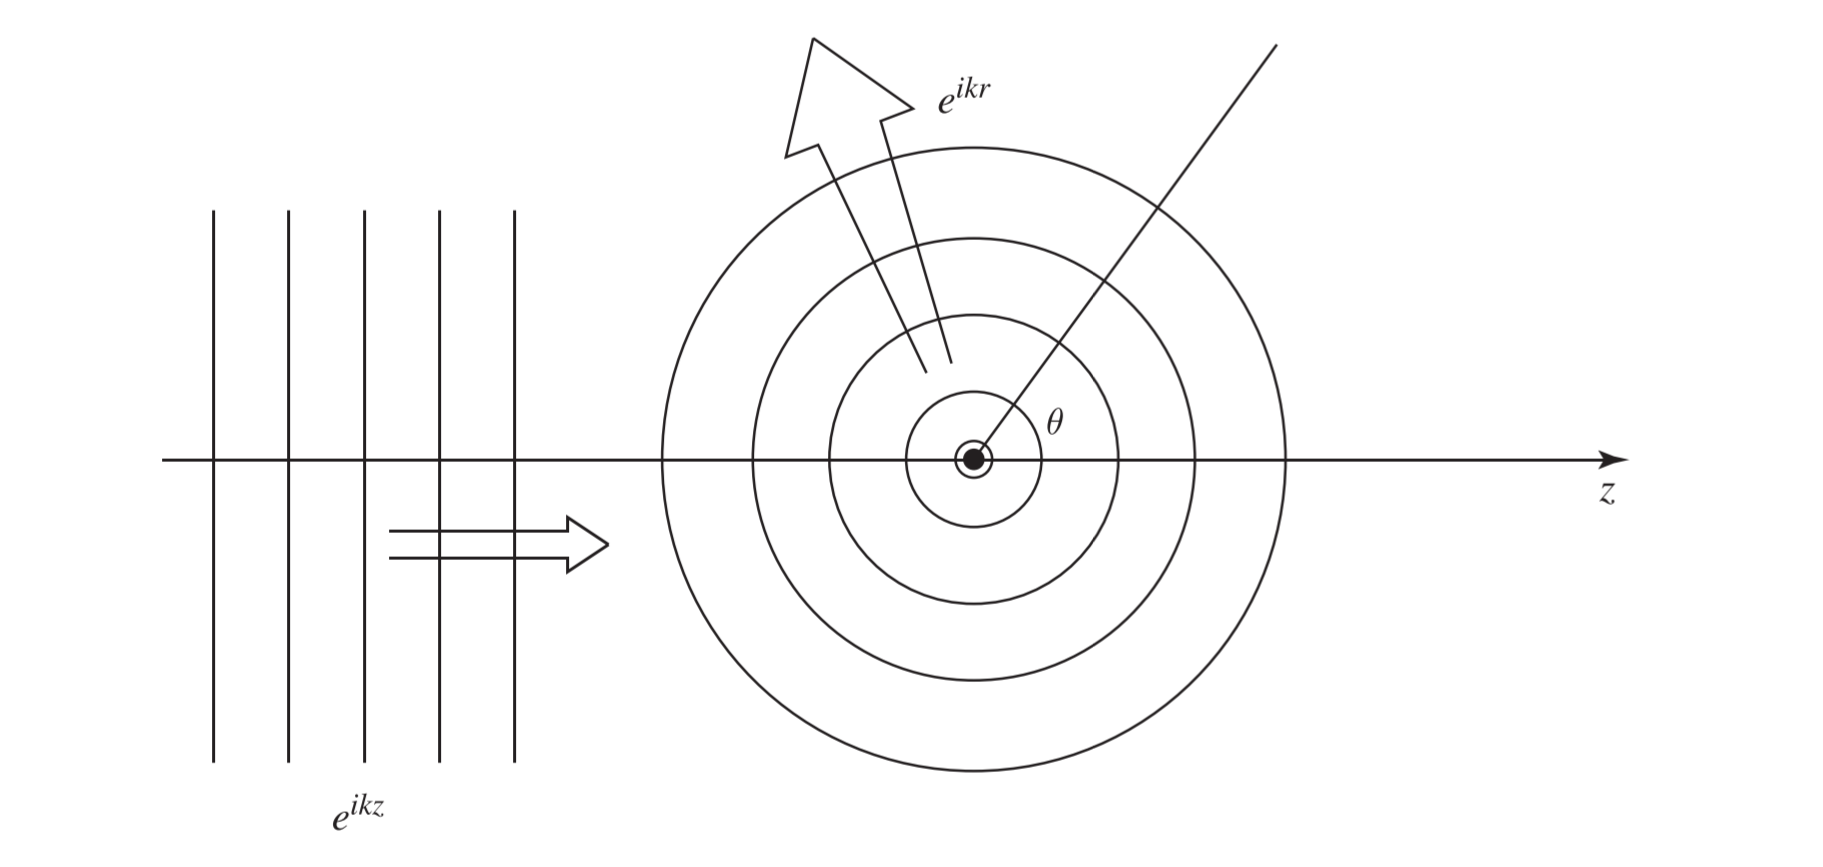
\includegraphics[width=\linewidth]{./images/Scattering1.png}
  				\caption{Quantum Scattering Schematics}
  				\label{fig:A Schematic of Quantum Scattering}
			\end{figure}
							
			\subsection{Quantum Scattering Theory}
			In quantum scattering theory we assume a wavefunction $\psi  = Ae^{ikz}$ moving in $z$ direction, encounters a potential and scatters in every direction as a spherical wave. Therefore the general answer that we are looking for is in the form:
			\begin{equation} 
			\psi(r,\theta) \approx A\bigg\{e^{ikz}+f(\theta)\frac{e^{ikr}}{r}\bigg\}
			\end{equation}

			So the whole problem is to find the scattering amplitude $f(\theta)$.  From out basic understandings from quantum mechanics we know that to find the probability of finding a particle at passing through a cross-section $d\sigma$ with a speed $v$ in time $dt$ is:
			$$
			dP =  |\psi_{\text{incident}}|^2 dV = |A|^2(v dt)d\sigma
			$$
			But this is equal to the probability that the particle scatters into the corresponding solid angle $d\Omega$:
			$$
			dP =|\psi_{\text{scattered}}|^2 dV = \frac{|A|^2|f|^2}{r^2}(vdt)r^2d\Omega
			$$
			from which it follows that $ d\sigma = |f|^2 d\Omega$ and thus:
			\begin{equation}
			D(\theta) = \frac{d\sigma}{d\Omega} = |f(\theta)|^2
			\end{equation}
			\begin{quotation}

			Evidently the differential cross-section (which is the quantity of interest to the experimentalist) is equal to the absolute square of the scattering amplitude (which is obtained by solving the Schrödinger equation). In the following sections we will study two techniques for calculating the scattering amplitude: partial wave analysis and the Born approximation.
			\end{quotation}
			As we know the Schrödinger equation for spherically symmetrical potential $V(r)$ admits the separable solution:
			$$
			\psi(r,\theta,\phi) = R(r)Y_\ell^m(\theta,\phi)
			$$
			where $u(r) =rR(r) $ satisfies the radial part of the equation:
			$$
			-\frac{\hbar^2}{2m}\frac{d^2u}{dr^2}+\bigg[V(r) + \frac{\hbar^2}{2m}\frac{\ell(\ell+1)}{r^2}\bigg]u = Eu
			$$
			if we look at the scattering from relatively large $r$ the second term in the right hand side is essentially zero and we are left with the equation:
			$$
			\frac{d^2u}{dr^2}\approx - k^2 u
			$$
			The general solution for this equation is:
			$$
			u(r) = Ce^{ikr}+De^{-ikr}
			$$
			the first term represents an outgoing particle and the second represents an incoming. For scattering therefore $D=0$. and therefore:
			$$
			R(r)\sim \frac{e^{ikr}}{r}
			$$
			This was the radiation zone, if we were in the Intermediate region (where $V$ can be ignored but the other term cannot) we would have:
			$$
			\frac{d^2u}{dr^2}-\frac{\ell(\ell+1)}{r^2}u = -k^2u
			$$
			and the general solution is a linear combination of spherical Bessel and Neumann functions but since we need a form of spherical wave (aka $\exp[ikr]$) we would write in the form of spherical Hankel function.
			$$
			h_\ell^{(1)} (x) = j_\ell(x) + in_\ell(x); \ \ h_\ell^{(2)}(x) = j_\ell(x) - in_\ell(x)
			$$
			then again the Hankel function of the second kind is in the form $\exp[-ikr]$ at large distances and therefore is not scattering result so we have only the Hankel function of the first kind:
			$$
			R(r) \sim h_\ell^{(1)} (kr) 
			$$
			The result would be in the form:
			$$
			\psi(r,\theta,\phi) = A\bigg\{e^{ikz} + \sum_{\ell,m} C_{\ell,m} h_\ell^{(1)}(kr)Y_\ell^{m}(\theta,\phi)\bigg\}
			$$
			but since we assumed a symmetrical potential it should not depend on $\phi$, leaving $m=0$
			$$
			Y_\ell^0 (\theta,\phi) = \sqrt\frac{2\ell+1}{4\pi} P_\ell(\cos\theta)
			$$
			the final wave function at intermediate region is:
			$$
			\psi(r,\theta) = A\bigg\{e^{ikz} + k\sum_{\ell=0}^\infty i^{\ell +1}(2\ell+1)a_\ell h_\ell^{(1)}(kr)P_\ell(\cos\theta)\bigg\}
			$$
			where we defined $C_\ell = i^{\ell+1}k\sqrt{4\pi(2\ell+1)}a_\ell$. now again for large $r$ we have $h_\ell^{(1)} = e^{ikr}/r$ and therefore:
			$$
			\psi(r,\theta)\approx A\bigg\{e^{ikz} + f(\theta)\frac{e^{ikr}}{r}\bigg\}
			$$
			where
			$$
			f(\theta) = \sum_{\ell=0}^{\infty}(2\ell+1)a_\ell P_\ell(\cos\theta)
			$$
			Now we have the differential cross-section:
			$$
			D(\theta) = |f(\theta)|^2=\sum_\ell\sum_{\ell'}(2\ell+1)(2\ell'+1)|a_\ell|^2P_\ell(\cos\theta)P_{\ell'}(\cos\theta)
			$$
			and using the orthogonality of the Legandre functions we have the total cross-section:
			$$
			\sigma = 4\pi\sum_{\ell=0}^\infty(2\ell+1)|a_\ell|^2
			$$
			\newpage
			\section{Light Propagation}
			\subsection{Basics of Light Propagation}
			\begin{itemize}
				\item \textbf{Absorption}: If the electron in atom is in \textit{resonance} with EM field, or in Quantum mechanics terms the energy of photon is suitable for electronic transition, light can be absorbed - energy of photon converted into higher potential energy of electron. 
				\item \textbf{Elastic Scattering}: Electrons in atoms are 'shaked' by oscillating $E$ field of light, Accelerated electrons then re-emit EM wave at the same frequency as incident light. Light scattered elastically has the same wavelength (frequency) as incident light. Each atom acts as a point-source of EM radiation. The resulting wave is a superposition of initial wave and all waves created by all atoms.
			\end{itemize}
			\subsubsection{Light Scattering}
			When Light encounters matter, matter not only re-emits light in the forward direction (leading to absorption and refractive index), but it also re-emits light in all other directions. This is called \textbf{Scattering}. Light scattering is happening everywhere. All molecules scatter light. Surfaces scatter light. It is the basis of nearly all optical phenomena.
			Scattering can be coherent or incoherent. This means that when light scatters in different angles they can have constructive or destructive interference.
			\begin{itemize}
			\item \textbf{Constructive interference (coherent)} Wave that combine \textbf{in phase} add up to relatively high irradiance.
			\item \textbf{Destructive interference (coherent} Waves that combine \textbf{$180\deg$ out of phase} cancel out yield zero irradiance. 
			\item \textbf{Incoherent addition} Waves that combine with lots of different phases nearly cancel out and yield very low irradiance.
			\end{itemize}
			
			
			
			
			
			
			
			
			
			

			
			
			
			
\end{document}
